
\section{Testovací prostředí}
Veškeré provedené testy proběhly na lokálním počítači s~operačním systémem Ubuntu 16.04,
na kterém zároveň proběhl vývoj nástroje. Systémové
prostředky dostupné pro testovaní byly: 4 jádra CPU, 8 GB RAM a 17 GB SSD disk.

Na počítači byl nasazen systém NEMEA a IoT brána BeeeOn, která byla rozšířena o~vytvořený detekční 
nástroj. Pro generování senzorových dat byly použity následující zařízení: BLE teplotní senzor (BeeWi), 
Z-Wave zásuvky (POPP a Fibaro) a virtuální senzory, které jsou dostupné pro testování
v~rámci BeeeOn brány.
Senzorová data přijímal testovací počítač, který měl připojený USB Z-Wave dongl (Aeotec) a integrované
BLE rozhraní.

\section{Způsoby nasazení}
Jako první byly testovány možnosti nasazení vytvořeného nástroje, který je možné používat
v~následujících režimech:

 \begin{itemize}
  \item \textbf{Lokální režim}
  
  V~lokální variantě byl použit pouze modul detektoru a kolektoru. Aby se nemusela pro každou 
  událost spouštět nová instance detektoru, byl využit již existující NEMEA modul \textit{Merger},
  který 
  dokáže jednotlivé UniRec zprávy spojit do jedné konsolidované. Způsob nasazení je zobrazen na Obrázku 
  \ref{obr.option1}.
  
  \begin{figure}[ht]
   \begin{center}
   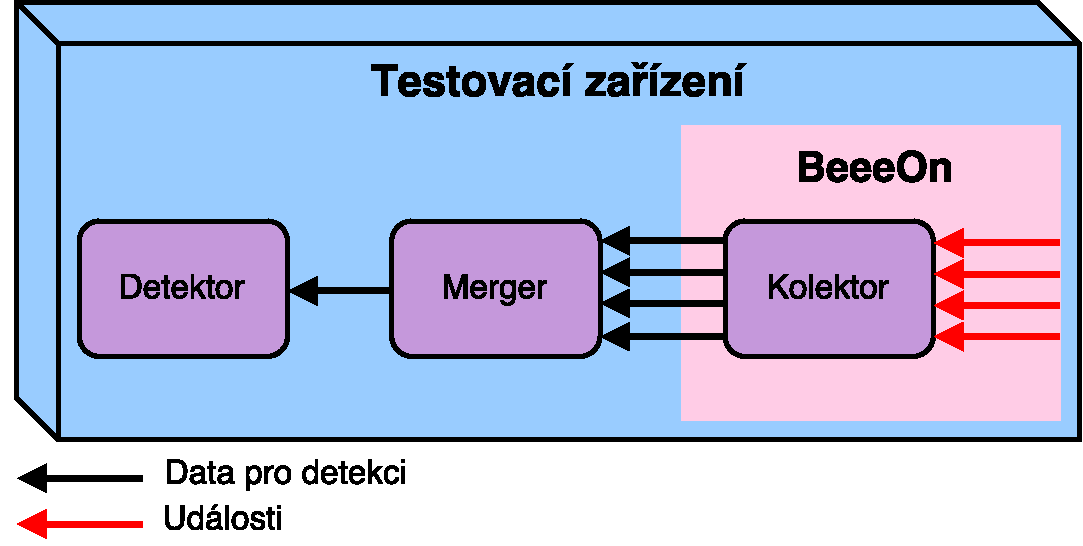
\includegraphics[scale=0.5]{pictures/deploy-option1}
   \caption{Lokální nasazení}
   \label{obr.option1}
   \end{center}
   \end{figure}
   
   Kolektor vždy odesílá dostupné události výstupními komunikačními rozhraními
   dle konfigurace brány.
   Exportovaná data přijímá NEMEA modul \textit{Merger}, který je spojuje a předává detektoru.
   
  \item \textbf{Oddělený režim} \label{externalMode}
  
  Druhý způsob nasazení byl také otestován na lokálním zařízení, protože lze využít lokálních
  soketů dostupných přes NEMEA framework. Provedení realizace je na Obrázku \ref{obr.option2}.
 
  \begin{figure}[ht]
   \begin{center}
   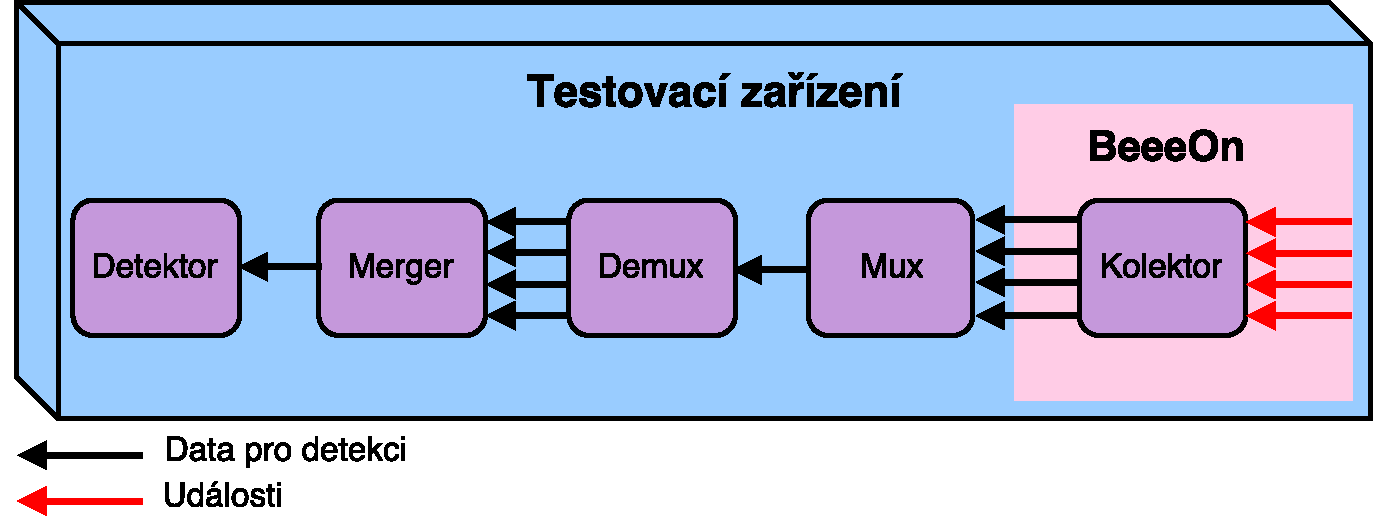
\includegraphics[scale=0.5]{pictures/deploy-option2}
   \caption{Oddělené nasazení}
   \label{obr.option2}
   \end{center}
   \end{figure}
   
   Složení komponent vychází z~prvního případu, který byl rozšířen o~moduly Mux a Demux, které 
   umí spojit a rozdělit přicházející komunikaci.
 \end{itemize}
 
Cílem testů bylo, aby detektor obdržel všechny odeslané zprávy z~kolektoru. Ověření bylo provedeno
spuštěním detektoru s~přepínačem \textit{-vv}, který zapne ladící výpisy druhé úrovně pro zobrazení 
přijatých UniRec polí. Výsledky obou případů byly úspěšné a všechna data byla přijata.

\section{Detekce scénářů útoků} \label{testAttack}
Velmi důležitou částí bylo otestování definovaných anomálií, které mohou reprezentovat skutečný
útok na sít. Tato sekce popisuje testy pro jednotlivé scénáře.

  \begin{enumerate}
    \item \textbf{Periodicita dat}
    
    Tento scénář nebylo nutné dělit na jednotlivé protokoly, protože popisuje obecné chování 
    připojených senzorů bez ohledu na technologii. Cílem bylo odhalit provoz, který porušuje
    očekávaný periodický průběh. V~rámci detekce nebyly potřebné naučené profily sítě, 
    ale využívalo se parametrů ze skupiny \textit{general} umožňujících periodické kontroly.
    
    První test byl určený na odhalení nepravidelného přijetí dat. Pro ověření byla použita událost
    \textit{onExport}, která poskytuje hodnoty získané ze senzorů, a v~konfiguračním souboru byla 
    aktivována pravidelná kontrola dat každých 8 sekund.
    
    Výsledek testu byl úspěšný. Pokud nebyla obdržena žádná data déle než 8 sekund, tak byly
    odeslány informace o~incidentu.
    
    Několik událostí poskytovaných branou BeeeOn jsou čistě periodické a~po uplynutí definovaného
    času vždy odešlou dostupné statistiky. Druhý test byl zaměřen na odhalení případu, kdy se 
    přijímané datové položky nemění, což může reprezentovat odpojení nebo ztrátu čidla. Pro 
    otestování byla zvolena událost \textit{onHciStats}, která získává informace o~provozu BLE sítě. 
    Dále byla v~konfiguračním souboru nastavena pravidelná kontrola dat na 7 sekund a maximálně 
    5 po sobě přijatých hodnot mohlo být stejných. 
    
    Výsledek byl pozitivní, protože při přijetí více než pěti stejných po sobě jdoucích
    hodnot byla detekována anomálie.
    
    \item \textbf{Množství přenášených zpráv}
    
    V~případě protokolu Z-Wave byly pro nasimulování anomálií použity dvě vzdáleně ovladatelné
    zásuvky. Obě mají k~dispozici ovládací tlačítko pro vypnutí a zapnutí zásuvky. Tímto způsobem
    byly generovány nové zprávy. Cílem tohoto scénáře bylo odhalit neočekávaný nárůst dat, a~proto
    byla zvolena detekční metoda, která hlídá tyto změny. V~rámci testu byly do profilu 
    vloženy všechny dostupné položky. Limitem pro ohlášení incidentu byl pětinásobný nárůst
    provozu. Délka časové řady byla nastavena na deset prvků a prvních jedenáct přijatých 
    zpráv bylo ignorováno, protože během nich bylo navazováno spojení.
    
    První detekce byla zaměřena na položku \textit{SOAFCount}, která určuje celkový počet 
    detekovaných zpráv.  
    Druhý scénář sledoval hodnotu \textit{receivedCount}, která reprezentuje počet přijatých zpráv od
    konkrétního čidla. 
    
    Pro BLE byla časová řada zkrácena na pět prvků, žádné zprávy nebyly ignorovány a limitem
    pro určení anomálie byl dvojnásobný nárůst dat.
    Test byl proveden pro položku \textit{rxBytes}, která určuje množství obdržených zpráv.
    Údaje byly vyčítány skriptem, který v~čase měnil četnost zaslaných požadavků o~data.
    
    Výsledky testů byly úspěšné a každá změna provozu byla odhalena. Průběh všech testovaných
    případů byl velmi podobný a lišil se jen typ události a způsob generování dat. Chování 
    jednotlivých položek profilu velmi ovlivňovala délka časové řady, která určovala 
    paměťové okno. Nejcitlivější položkou na změnu byl rozptyl, který výrazně zvyšoval
    svou hodnotu při vložení vyššího čísla. K~častým výchylkám docházelo i v~případě průměru. 
    Méně frekventované změny nastávaly u~mediánu, který nejvíce využíval délky časové řady. 
    Nejmenších odlišností dosahoval klouzavý průměr, protože ve své hodnotě obsahuje i data
    mimo aktuální časové okno.

    \item \textbf{Limity senzorových hodnot}
    
    Pro tento scénář byla použita data vygenerována virtuálními senzory, které jsou dostupné
    v~rámci brány BeeeOn. Do konfiguračního profilu byly vloženy všechny položky, pro které
    byly specifikovány parametry pro očekávané soft a hard limity. Cílem scénáře bylo odhalení
    změn v~aktuálním profilu provozu, které porušují předepsané limity. 
    
    Výsledek detekce splnil očekávání a nepovolené změny byly úspěšně detekovány. Chování 
    jednotlivých položek profilu se shodovalo s~předchozím scénářem.
    
    \item \textbf{Kvalita přenosového kanálu}
    
    Cílem tohoto případu užití bylo detekování změny kvality přenosového kanálu. Pro Z-Wave jsou 
    k~tomuto účelu vhodné položky \textit{lastResponseRTT} a \textit{dropped}. Údaj
    \textit{lastResponseRTT} je součástí události \textit{onNodeStats} a 
    \textit{dropped} je obsažen v~\textit{onDriverStats}. Z~tohoto důvodu byl při generování dat použit
    NEMEA modul \textit{Merger}, který spojil dvě různě události do jedné. Zároveň bylo nutné
    v~konfiguračním souboru
     popsat obě hodnoty. V~případě \textit{lastResponseRTT} byla jako anomálie označena
    hodnota klouzavého průměru časové řady přesahující dvojnásobek vzorového profilu a nebo byla nižší
    než polovina stanoveného klouzavého průměru. Pro položku \textit{dropped} bylo jako incident považováno
    libovolné zvětšení klouzavého mediánu. Proto byla velikost časového okna rovna jedné a hard limitu byl
    nastaven na jedna. 
    
    Jelikož došlo ke spojení dvou různých událostí, kde \textit{onNodeStats}
    umožňuje získat informace pro jednotlivé senzory a \textit{onDriverStats} pro celou síť, 
    tak výsledkem byla událost poskytující informace pro každý koncový prvek. Z~tohoto důvodu 
    musel být v~konfiguraci uveden v~rámci klíče identifikátor příslušných zařízení určených k~analýze.
    
    Výstupy detekce se shodovaly s~předpoklady, a proto byl výsledek testu úspěšný. V~současné
    době se zatím nepodařilo připravit zkušební prostředí, ve které by bylo možné otestovat
    rušení kanálu, a tím ovlivnit hodnotu \textit{lastResponseRTT}. Pro účely otestování 
    detekce však byla postačující ruční úprava dat v~souboru se zachyceným provozem. 
    
    V~případě BLE by se využily položky \textit{rxErrors} nebo \textit{txErrors} a nastavení 
    detekce by bylo shodné s~\textit{lastResponseRTT}. Vzhledem k~tomu, že by došlo jen 
    ke změně názvu klíče v~konfiguračním souboru, tento test nebyl proveden.
    
    \item \textbf{Konektivita}
    
    Pro ověření posledního scénáře lze využít poznatků z~předchozích testů. Ztráta konektivity
    může být způsobena neobdržením očekávané události a to lze detekovat pomocí periodicity dat.
    Druhým způsobem je výrazné zhoršení statistik přenosového kanálu, které byly zpracovány
    v~předchozím případu užití.
  \end{enumerate}
  
  Ověření definovaných scénářů umožnilo otestování správné funkcionality vytvořeného detekčního
  systému a zároveň byla sestavena množina informací, kterou je nutné sledovat k~získání 
  přehledu o~stavu sítě.
  
  Vygenerovaný provoz, na kterém byly jednotlivé případy užití otestovány je uložen i s~nalezenými
  anomáliemi a konfiguračním souborem na přiloženém CD. V~případě testu periodicity dat nebylo možné záznam 
  komunikace uložit, protože použitá detekce využívá aktuální čas. Z~tohoto důvodu 
  byl do souboru místo záznamu uložen popis, jak takový provoz vygenerovat.

\section{Test exportu dat}
Identifikované scénáře útoků otestovaly většinu funkcí detekčního systému. Vytvořený nástroj
ovšem poskytuje i možnost pravidelného exportu definovaných položek aktuálního profilu, a tím 
vytváří informace pro další pokročilejší detekce. 

Sada testů ověřila, že vypočítané části profilu lze spolehlivě exportovat. Výsledek byl tedy
pozitivní.

\section{Měření položek profilu}
Již v~sekci \ref{testAttack} bylo možné sledovat odlišné chování 
jednotlivých částí profilu. V~této sekci je provedeno vyhodnocení každé z~nich. Veškeré 
měření probíhalo nad stejným provozem, kde byly zprávy generovány každé tři sekundy a~pravidelné
události chodily každých pět sekund. Incidenty byly reprezentovány nárůstem sledovaného provozu.

Tabulka \ref{tab.tab1} zobrazuje pro každou položku profilu počet detekovaných anomálií 
s~rostoucí velikostí časové řady. Její vyšší rozměry nejvíce stabilizovaly klouzavý medián, protože jeho počty
incidentů klesly se zvyšující se délkou. Zároveň z~jeho grafu \ref{obr.progressMedian} lze vidět,
že začátek anomálií odhalil vždy jako poslední a jejich doba trvání byla nejkratší. 

S~větší časovou řadou bylo možné uchovat i více hodnot, a 
tím se detekovalo více událostí v~rámci klouzavého průměru a rozptylu. Začátky i konce rozpoznání incidentů
byly u~obou položek velmi podobné. Jediným rozdílem u~klouzavého rozptylu bylo, že při stabilním 
nárůstu sledované položky může jeho hodnota po uplynutí časového okna opět klesnout do bezpečného pásma. 
Graf průběhu \ref{obr.progressStandardDeviation} pro větší přehlednost nezobrazuje klouzavý rozptyl, ale 
klouzavou směrodatnou odchylku. 

Průměr jako jediný nebyl závislý na časovém okně. Ovšem s~rostoucí délkou řady 
byla delší i doba učení, při které byla vždy stanovena lehce odlišná hodnota vzorového
profilu a mezních limitů. Při provedeném měření se vždy s~delším paměťovým oknem vzorové hodnoty mírně 
zvýšily.
Na základě těchto předpokladů lze v~jeho grafu \ref{obr.progressCumAverage}
vidět pomalé klesání, díky kterým byly incidenty detekovány nejdelší dobu. Zároveň dle očekávání velikost 
časového okna nemá vliv na počet detekovaných anomálií.



\begin{table}[ht]
  \begin{center}
  \begin{tabular}{|C{1.7cm}|C{1.7cm}|C{1.7cm}|C{1.7cm}|C{1.7cm}|}
    \hline 
   \thead{velikost\\ časového\\ okna} & \thead{klouzavý\\ medián} & \thead{klouzavý\\ rozptyl} & \thead{klouzavý\\ průměr} & \thead{průměr}\\
   \hline 
   \hline 
    1 & 26 & 0 & 26 & 26\\
    \hline
    3 & 26 & 30 & 30 & 90\\
    \hline
    5 & 26 & 34 & 32 & 89\\
    \hline
    10 &  26 & 44 & 40 & 89\\
    \hline
    15 & 19 & 54 & 48 & 89\\
    \hline
    20 & 19 & 62 & 56 & 89\\
    \hline
   \end{tabular}
   \caption{Tabulka obsahuje počty detekovaných anomálií s~rostoucí délkou časového okna} 
   \label{tab.tab1}
  \end{center}   
    \end{table}

    \begin{figure}[ht]
   \begin{center}
   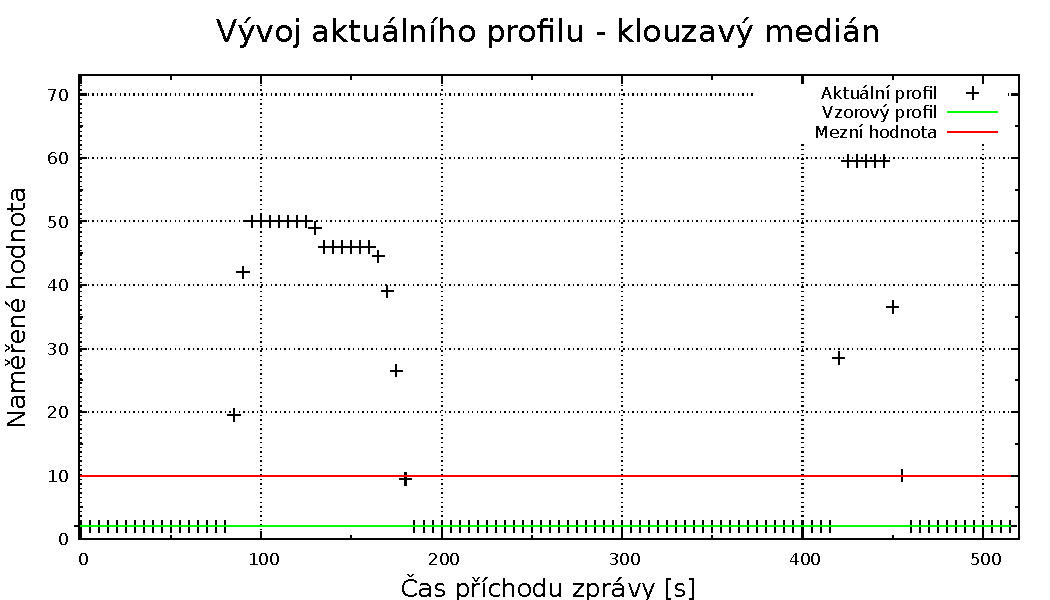
\includegraphics[scale=0.7]{pictures/moving_median_progress}
   \caption{Graf vývoje klouzavého mediánu s~časovou řadou délky 10}
   \label{obr.progressMedian}
   \end{center}
   \end{figure}
   
   \begin{figure}[ht]
   \begin{center}
   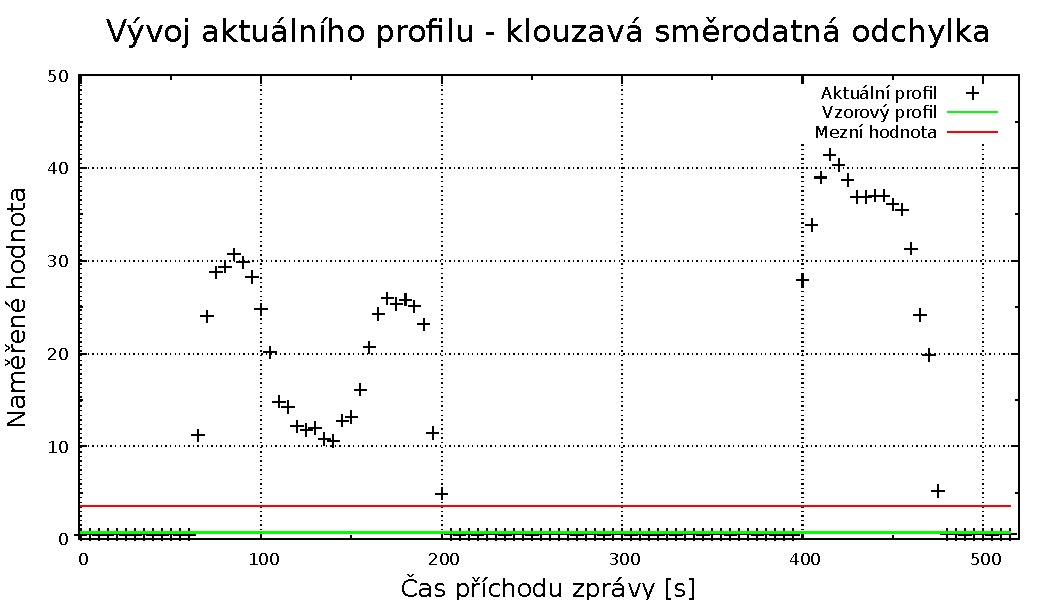
\includegraphics[scale=0.7]{pictures/moving_standard_deviation_progress}
   \caption{Graf vývoje klouzavé směrodatné odchylky s~časovou řadou o délce 10}
   \label{obr.progressStandardDeviation}
   \end{center}
   \end{figure}
    
  \begin{figure}[ht]
   \begin{center}
   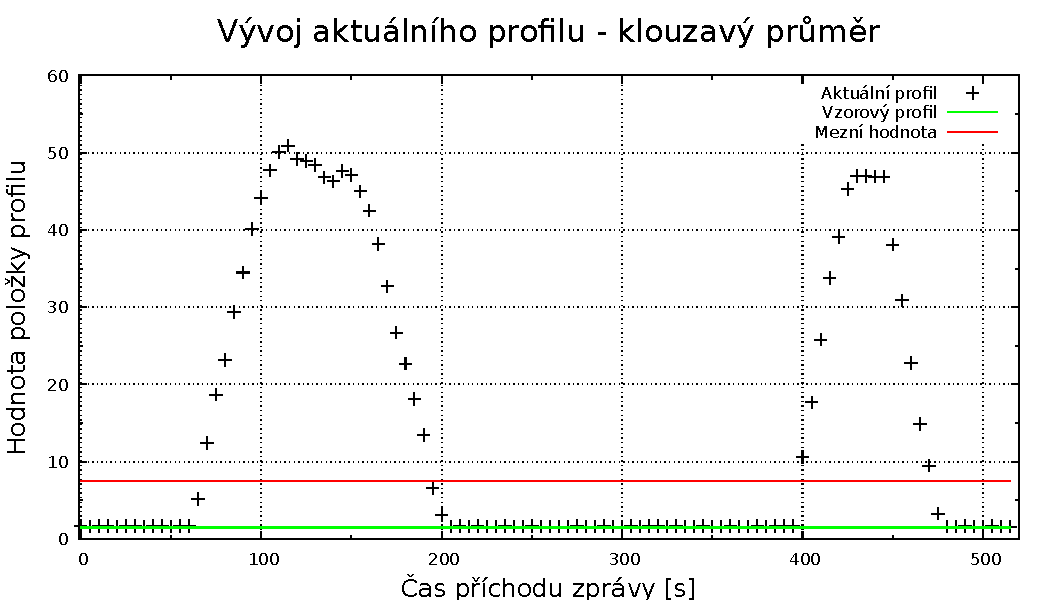
\includegraphics[scale=0.7]{pictures/moving_average_progress}
   \caption{Graf vývoje klouzavého průměru s~časovou řadou délky 10}
   \label{obr.progressAverage}
   \end{center}
   \end{figure}
   
   \begin{figure}[ht]
   \begin{center}
   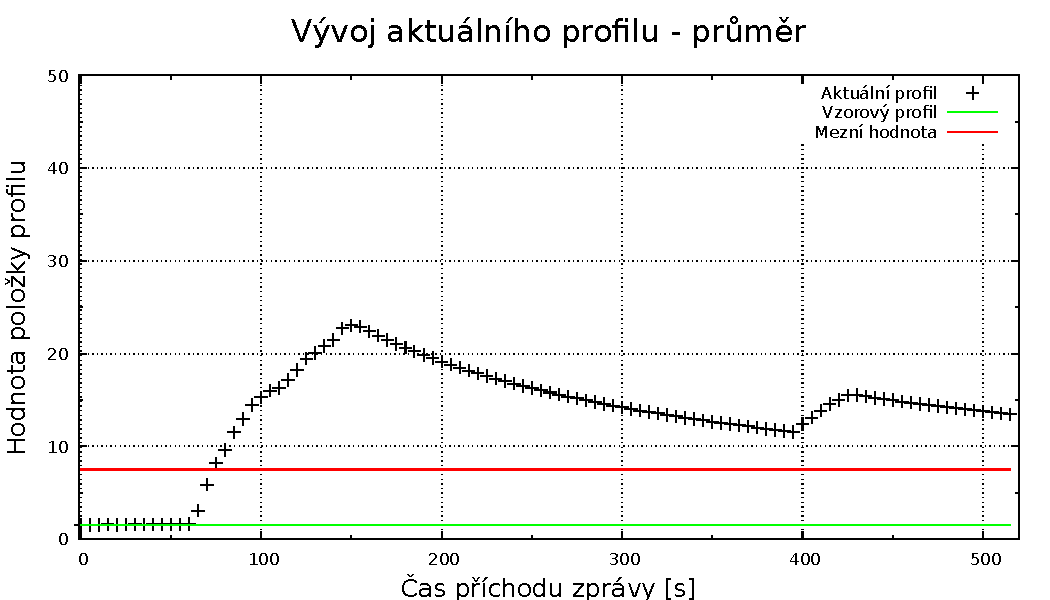
\includegraphics[scale=0.7]{pictures/average_progress}
   \caption{Graf vývoje průměru s~časovou řadou délky 10}
   \label{obr.progressCumAverage}
   \end{center}
   \end{figure}